\documentclass[tikz, border=0px]{standalone}
\usepackage{tikz}
\usetikzlibrary{shapes,arrows}

\tikzstyle{startstop} = [rectangle,rounded corners,minimum width=3cm,minimum height=1cm,align=center,draw=black, text width=2.5cm, fill=green!30]

\tikzstyle{therapy} = [trapezium, trapezium left angle =70, trapezium right angle=110, minimum width=2cm, minimum height = 1cm, centered,draw=black,align=center, text width=2cm, fill=orange!30]

\tikzstyle{decision} = [diamond, minimum width = 3cm, minimum height = 3cm, text centered, draw=black, text width = 2cm,align=center,fill=blue!30]

\tikzstyle{arrow} = [thick, ->, >=stealth]
\tikzstyle{doublearrow} = [<->, thick, >=stealth]

\begin{document}
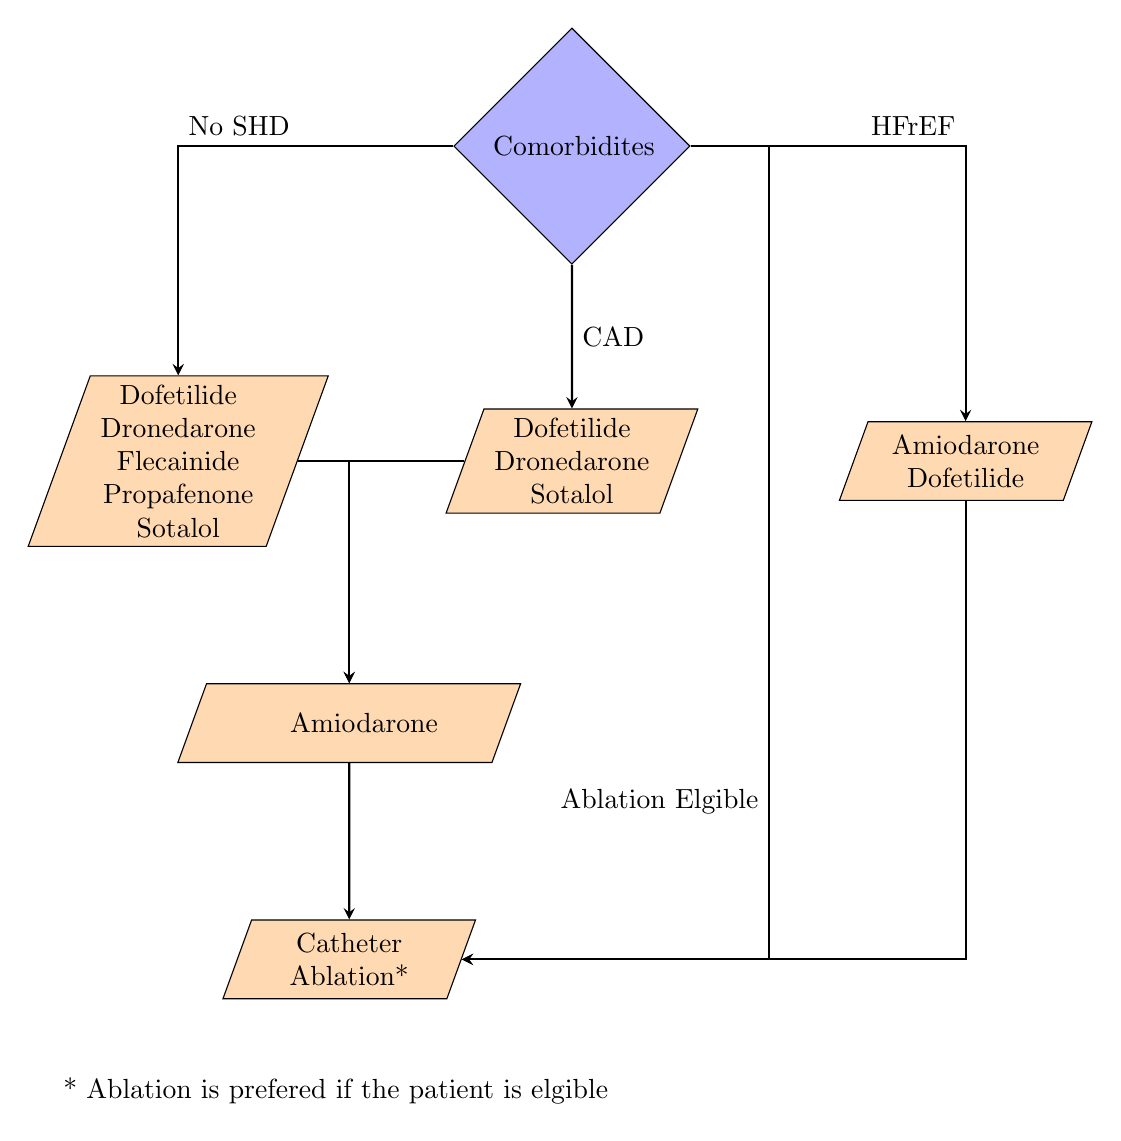
\begin{tikzpicture}[node distance=4cm]

\node (start) [decision] {Comorbidites};
\node (healthyDrugs) [therapy, below of=start, xshift=-5cm] {Dofetilide Dronedarone Flecainide Propafenone Sotalol};
\node (cadDrugs) [therapy, below of=start] {Dofetilide Dronedarone Sotalol};
\node (HFrEFDrugs) [therapy, below of=start, xshift=5cm] {Amiodarone Dofetilide};
\node(amiodarone) [therapy, below left of=cadDrugs, text width=1.5cm, yshift=-0.5cm] {Amiodarone}; 
\node(ablation) [therapy, below of=amiodarone, text width=2cm, yshift=1cm] {Catheter Ablation*};

\node [rectangle, below of=start, xshift=-3cm, yshift=-8cm] {* Ablation is prefered if the patient is elgible};

\draw [arrow] (start) -| node[anchor=south west] {No SHD} (healthyDrugs);
\draw [arrow] (start) -- node[anchor=west] {CAD} (cadDrugs);
\draw [arrow] (start) -| node[anchor=south east] {HFrEF} (HFrEFDrugs);
\draw [arrow] (healthyDrugs) -| (amiodarone);
\draw [arrow] (cadDrugs) -| (amiodarone);
\draw [arrow] (amiodarone) -- (ablation);
\draw [arrow] (HFrEFDrugs) |- (ablation);
\draw [arrow] (start) -- ++(2.5cm,0) |- node [anchor = east, yshift=2cm] {Ablation Elgible} (ablation);


\end{tikzpicture}
\end{document}